\documentclass{article}
\usepackage{amsmath}
\usepackage{bm}
\usepackage{graphicx}
\usepackage{appendix}

\title{Bayesian update rule leads to information theoretically optimal evolution\\ \begin{normalsize}Why to help those weaker than you\end{normalsize} }
\author{Tomas Ukkonen\\ \textrm{tomas.ukkonen@iki.fi} }
\date{\today}
\begin{document}
\maketitle

\section{Introduction} \label{introduction}

Evolution can be underatood as an optimization process that tries to collect information  \cite{infobook03} as well as possible from  an environment in order to increase fitness. One can think a current population as the distribution of genes $p(\mathbf{x})$ and then have a fitness function where outcomes are uncertain and defined as the probability of fitness $p(\mathbf{f}|\mathbf{x})$. It is then possible to use the bayes rule \cite{bdanalysis03} to calculate the posterior distribution of good genes $p(\mathbf{x}|\mathbf{f})$ given the fitness outcomes $\mathbf{f}$.

\begin{equation}
\label{bayesupdate}
p(\mathbf{x}|\mathbf{f}) \propto p(\mathbf{f}|\mathbf{x})p(\mathbf{x}) \end{equation}

\begin{equation}
\label{entropyupdate}
H(\mathbf{X}|\mathbf{F}) = H(\mathbf{X}) - I(\mathbf{X};\mathbf{F})
\end{equation}

The bayesian update rule is information theoretically optimal meaning information is gained as fast as possible from the environment.

\section{Information Theory}

It is easy to prove equation \ref{entropyupdate} is correct from bayesian update equation \ref{bayesupdate}.

\begin{equation*}
\begin{aligned}
  p(\bm{x}|\bm{f})p(\bm{f}) &= p(\bm{f}|\bm{x})p(\bm{x})\\
  log(p(\bm{x}|\bm{f})) + log(p(\bm{f})) &= log(p(\bm{f},\bm{x}))\\
  E_{\bm{x}\bm{f}}\{log(p(\bm{x}|\bm{f})) + log(p(\bm{f}))\} &= E_{\bm{x}\bm{f}}\{log(p(\bm{f},\bm{x}))\}\\  
  H(\bm{X}|\bm{F})+H(\bm{F}) &= H(\bm{X},\bm{F}) \\
  H(\bm{X}|\bm{F}) &= H(\bm{X},\bm{F}) - H(\bm{F}) \\
  H(\bm{X}|\bm{F}) &= H(\bm{X}) - I(\bm{X};\bm{F})
\end{aligned}
\end{equation*}

However, the reverse is not necessarily true.  There may be non-bayesian methods to process data that are information theoretically optimal as well.

\section{Metropolis-Hastings and Evolution}

A paper published on 2003 \cite{strens03} describes methodology to combine genetic algorithms and MCMC sampling. However, the author do not establish overall framework to combine bayesian inference, genetic algoritms and sampling discussed here.

Metropolis-Hastings method \cite{bdanalysis03} produces samples $\mathbf{x}_{t+1}$ from any target distribution $P(\mathbf{x})$ by drawing samples $\mathbf{x}'$ from auxiliary distribution $g(\mathbf{x}'|\mathbf{x}_t)$ and then accepting samples $\mathbf{x}'$ with probability $a$,

\begin{equation}
  \label{mcmcsampling1}
  a = max(1, \frac{P(\mathbf{x}')}{P(\mathbf{x}_t)} \frac{g(\mathbf{x}_t|\mathbf{x}')}{g(\mathbf{x}'|\mathbf{x}_t)})
\end{equation}.

To mimic the evolution, we draw initial $\mathbf{x}'$ from a bayesian prior distribution $g(\mathbf{x}'|\mathbf{x}_t) = p(\mathbf{x}')$ and want our target distribution to be the posterior $P(\mathbf{x}) = p(\mathbf{x}|\mathbf{f})$. Straightforward calculation then shows that our accepting probability $a$ becomes

\begin{equation}
  \label{mcmcsampling2}
  a = max(1, \frac{p(\mathbf{f}|\mathbf{x}')}{p(\mathbf{f}|\mathbf{x}_t)})
\end{equation}

So we always accept cases when a fitness likelihood ratio increases and when it worsens, we still accept those cases with probability $a$. This mechanism, of 1) drawing samples from a prior $p(\mathbf{x})$, and then 2) accepting new samples according to the fitness likelihood ratio $a$, will create proper samples from the bayesian posterior. In practice, we have samples from $p(\mathbf{x})$ and we now need to generate more samples (``sex'') having the same distribution and then put them through fitness likelihood ratio (``soft competition'') so we get the proper posterior.
 
To further simplify generation of similarly distributed genomes through ``sex'', it is assumed that genes are independently distributed,

\begin{equation}
  p(x_1,x_2,...,x_n)=\prod_{i=1}^{N}p(x_i)
\end{equation}

This will then allow generating new similarly distributed genome from the two randomly chosen ``parent genomes'' $p(\mathbf{x}^k)$ and $p(\mathbf{x}^l)$ by choosing genes from either one

\begin{equation}
  p(\mathbf{x}^{new})=\prod_{i=1}^{N}p(x_i^{random(k,l)})
\end{equation}

A pool of $M$ individuals from the previous generation $\{\mathbf{x}_t\}$ is then generated and updated according to the modified Metropolis-Hastings sampling rule outlined above.


\section{Experiments} \label{experiments}

\subsection{Experiment 1}

To investigate adaptation speed of our modified Metropolis-Hastings algorithm, $N=100$ bits long genome and a random initial population of size $M=100$ was generated where each bit in on position increases fitness score by one. The data likelihood probabilities for fitness was chosen to be binomial distribution 

\begin{equation}
  p(f|\mathbf{x}) = \binom{N}{f} p^{f}(1-p)^{N-f}, p = \frac{sum(\mathbf{x})}{N}
\end{equation}

and the observed fitness values $f$ were drawn from the same distribution as $p(f|\mathbf{x}')$. In our experiment, the acceptance probability $a$ was altered to test the speed of adaptation by either increasing ($k=0.10$) or reducing ($k=10$) acceptance probability for selecting worse solution or keeping it unaltered ($k=1$), 

\begin{equation}
  \label{mcmcsampling3}
  a(k) = max(1, \frac{p(f|\mathbf{x}')}{p(f|\mathbf{x}_t)})^{k}
\end{equation}

Computer simulations were run 30 times, each time simulating 1000 generations. In our experiments, the highest fitness declined as the number of generations increased (Figure \ref{fig:experiment1f4}) while the average fitness within population increased only slightly (Figure \ref{fig:experiment1f3}) before converging to the same value. Direct inspection of binary genomes revealed that the whole population has become homogenous and each individual had the same genome. The failure to find the optimal solution from $2^{100}$ possible cases was not surprising and the results clearly show unscalability of the quite naive method of generating new genomes to gigantic problem spaces.

\begin{figure}

\centering
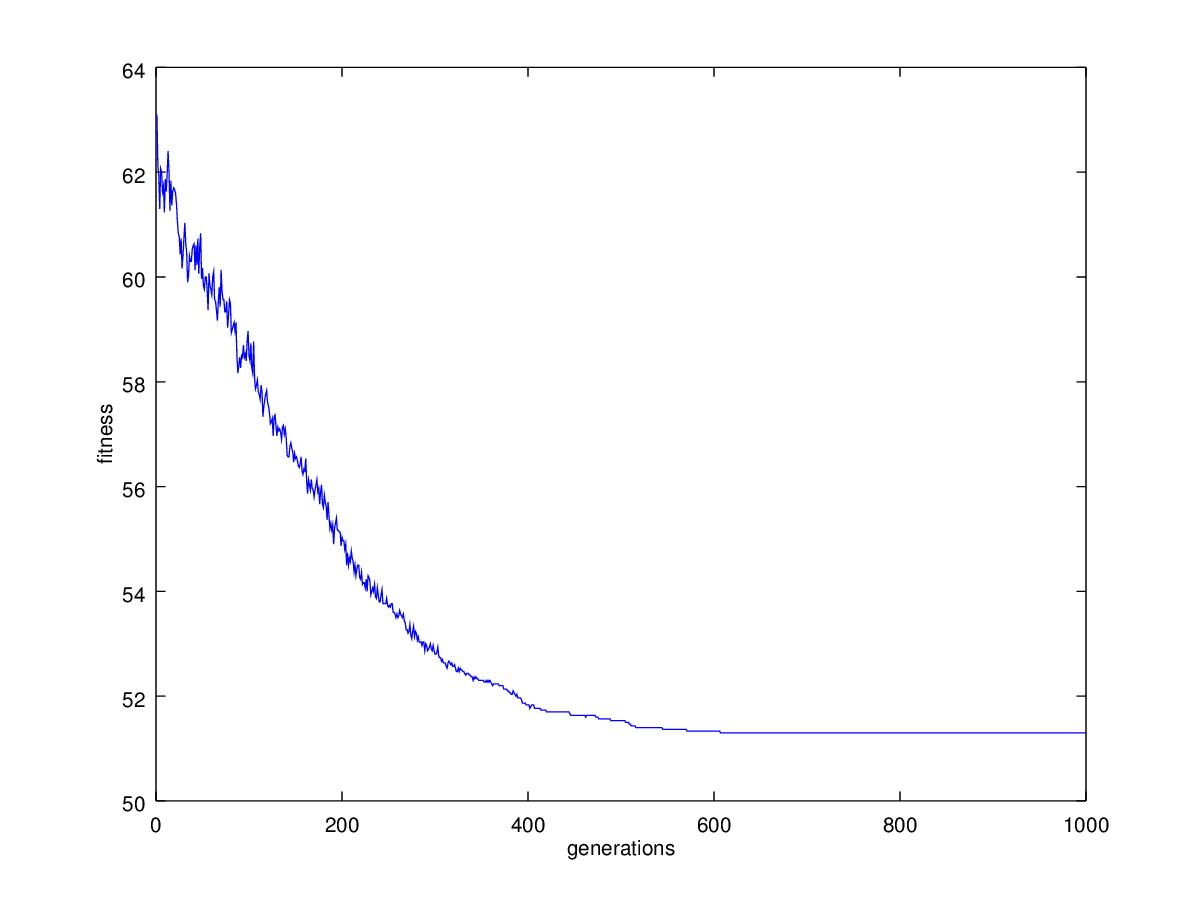
\includegraphics[keepaspectratio,width=0.9\textwidth]{experiment1figure4.jpg}

\caption{Average highest fitness ($k = 1$)}

\label{fig:experiment1f4}

\end{figure}

\begin{figure}

\centering
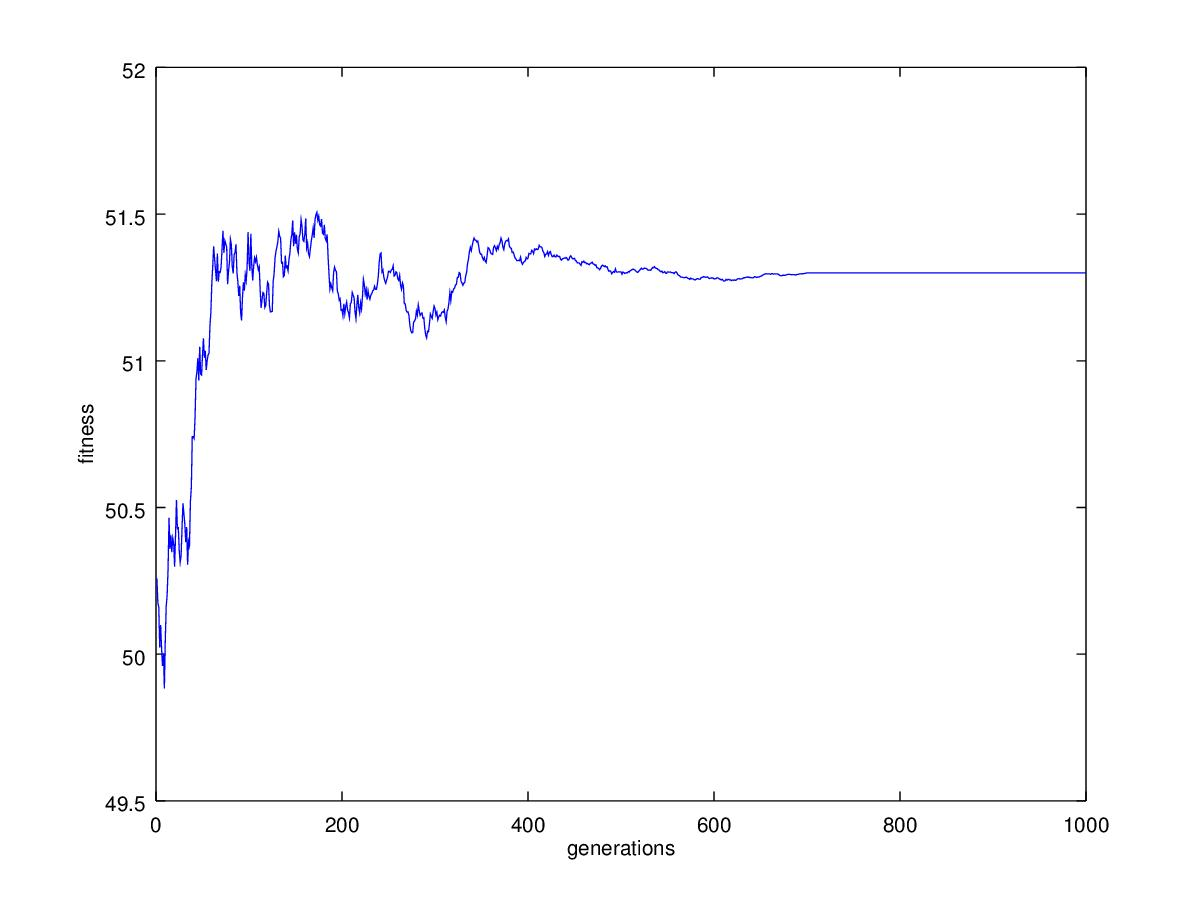
\includegraphics[keepaspectratio,width=0.9\textwidth]{experiment1figure3.jpg}

\caption{Average population fitness ($k = 1$)}

\label{fig:experiment1f3}

\end{figure}


\subsection{Mutations}

Because choosing of the bits from the parent genomes randomly cannot invent anything new and is destined repeat same solutions,
a ``mutation'' operation was added. The methodology assigns each bit a probability $[0,1]$ of it being on or off.


\section{Fitness} \label{fitness}

Information is gained from the environment according to $I(\mathbf{F};\mathbf{X}) < H(\mathbf{F})+H(\mathbf{X})$. This means information reduction   
$\frac{\partial H(\mathbf{X}|\mathbf{F})}{\partial \mathbf{F} }$
 is bounded by entropy of fitness $H(\mathbf{F})$ and individuals maximizing entropy $H(\mathbf{F})$ has $p$ value $1/e \approx 0.37$  (Figure \ref{fig:plogp}). This means individuals can be probabilistically divided into just 3 equally sized groups according to their fitness $\mathbf{F}$ and it does not make sense to try to decide fitness very accurately.

\begin{figure}

\centering
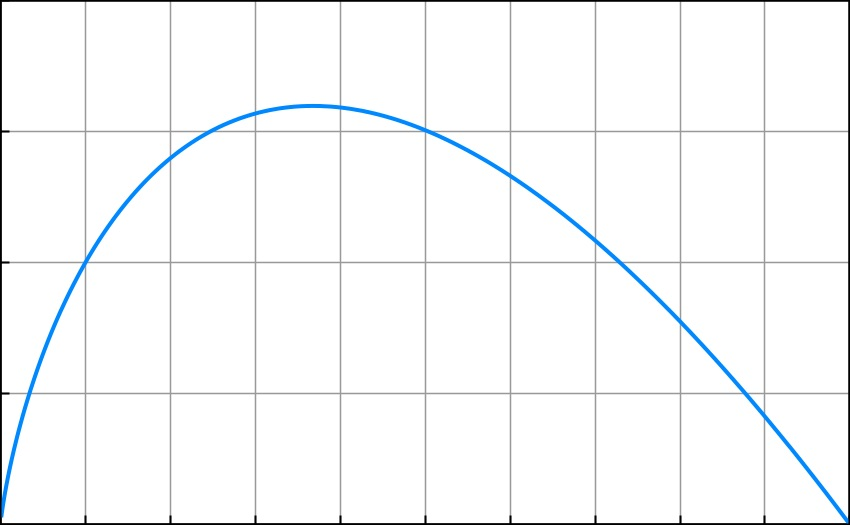
\includegraphics[keepaspectratio,width=0.9\textwidth]{plogp.jpg}

\caption{Value of $p*log(1/p)$}

\label{fig:plogp}

\end{figure}


One way to measure fitness without fighting and killing is to only  measure life expectancy. Genes are  collected from individuals at the birth and those that had the longest lifespans generate most new children.

Because fitness should be only measured inprecisely. It is maybe correct to divide individuals into three age groups and deny descendants from the first (0-20), then probabilistically allow it for the second (20-40) and maybe always allow it for the third equally sized group (40-60). DNA could be collected from the older persons to give birth to the grandchildren, or it is maybe naturally impossible because of too high fitness and need to keep evolution in the search mode.

\section{Modelling (work in progress)} \label{modelling}

We use probabilistic bayesian modelling  \cite{bdanalysis03} as a basis of our models. In order to measure changes in entropy, we estimate $H(\bm{X})$  from samples representing prior and posterior distributions \cite{entropy01}.


\subsection{Precise Life Expectancy Model}

In the first model, the life expectancy of individual's genes $\bm{p}|\bm{\alpha},\bm{\beta} \sim Beta(\bm{\alpha},\bm{\beta})$ is assumed to be directly related to goodness of  genes $\bm{g} \sim Normal(\bm{0}, \bm{I})$. Life expectancy $l$ is therefore $\bm{g}^T \bm{p}$ and for the large number genes G it is normally distributed $Normal(\mu_l,\sigma_l)$ leading to a model which disallows descendants for aged individuals.

\begin{equation}
\label{eq:lifeexp1}
\begin{aligned}
\mu_l &= E_p[\bm{g}^T \bm{p}] = \bm{g}^T \bm{\mu}_p \\
\sigma_l^2 &= Var_p[\bm{g}^T \bm{p}] = \bm{g}^T \bm{\Sigma}_p \bm{g} = \bm{g}^T \bm{I}(\bm{\alpha},\bm{\beta}) \bm{g}
\end{aligned}
\end{equation}

This normal distribution is only approximation as the life expectancy, or the fitness, varies between $[-L,L]$ where $L = \|\bm{g}\|^2$. For the population update, we use bayes rule (and choose initially a flat prior $p(\bm{\alpha},\bm{\beta}) \propto 1$) leading to an  integral: 

\begin{equation}
\begin{aligned}
p(\bm{\alpha},\bm{\beta}|\mathbf{g}) &\propto \int p(l|\bm{\alpha},\bm{\beta},\mathbf{g},\mathbf{p}) p(\mathbf{p}|\bm{\alpha},\bm{\beta}) p(\bm{\alpha},\bm{\beta}) \, \mathrm{d}\mathbf{p} \\ 
p(\bm{\alpha},\bm{\beta}|\bm{g}) &\propto \int Normal(\bm{g}^T \bm{p} | \mu_l, \sigma_l) Beta(\bm{p}|\bm{\alpha},\bm{\beta}) p(\bm{\alpha},\bm{\beta})  \, \mathrm{d}\bm{p}
\label{eq:bupdate2}
\end{aligned}
\end{equation}

This population update rule can be applied repeatedly by using the previous $\bm{\alpha}$s and $\bm{\beta}$s as the new single valued priors (impulse peaks) and assuming fixed $\bm{g}$.

\begin{figure}

\centering
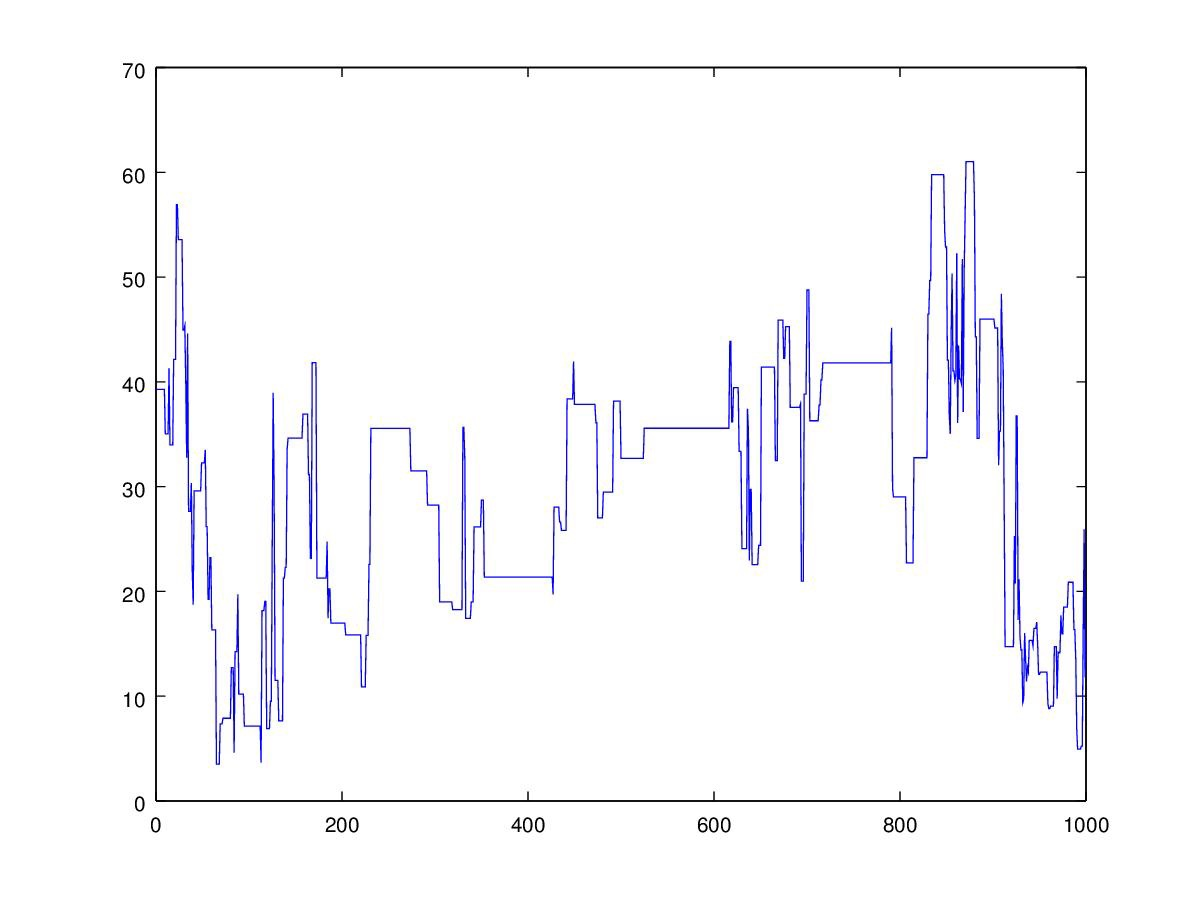
\includegraphics[keepaspectratio,width=0.9\textwidth]{method1.jpg}

\caption{Model 1: Angle between $\bm{g}$ and $\bm{p}$ between successive iterations}

\label{fig:method1}

\end{figure}


\subsection{Imprecise Life Expectancy Model}
\label{dlifesec2}

Based on the discussion in section \ref{fitness}, a slightly altered model can be attempted so that life expectancy is discretized into three equally-sized bins. We calculate $\sigma_l$ using the equation \ref{eq:lifeexp1},  discretize data to intervals $]-\infty,0.5\sigma_l]$, $]-0.5\sigma_l,+0.5\sigma_l[$ and $[+0.5\sigma_l,+\infty[$ and try to use $Dirichlet(\bm{\gamma})$ distribution for data likelihood.

\subsection{Tournament Life Expectancy Model}

In the third model, individuals compete against each other and indirectly collect information from the environment through $K$ tournaments between different individuals. We simulate results of these tournaments by assuming life expectancy $l$ dictates results of tournaments between other individuals. During each year/step k, individual can either survive $q$ or fail $(1-q)$ leading to the familiar distribution 

\begin{equation}
p(k) \propto q^{k-1} (1-q)
\end{equation}

This gives success probabilities $Beta(k,2)$ for each individual when competing against others. The competition can then lead to three different outcomes:  $(1,0)$ indicating a victory, $(0,1)$ indicating a loss or $\{(0,0), (1,1)\}$ meaning a tie. We ignore ties (no information), so data $(N,k)$ likelihood has the $Binomial(k|N, q)$ form where probability $q$ has a flat $Beta$ prior. This model gives clear preference to aged individuals meaning they are more likely to have descendants than younger ones.

We can again write the generic formula for updating population distribution

\begin{equation}
p(\bm{\alpha},\bm{\beta}|\mathbf{g}) \propto \int p(k|\bm{\alpha},\bm{\beta},\mathbf{g},\mathbf{p},q) p(\mathbf{p}|\bm{\alpha},\bm{\beta}) p(\bm{\alpha},\bm{\beta})p(q) \, \mathrm{d}\mathbf{p} \,  \mathrm{d}q
\end{equation}

where k is calculated from tournament simulations.

\subsection{Tournament Life Expectancy Model with Age}

To remedy the modelling problem leading to unnatural preference of aged individuals, a fourth model is attempted. Here we use discretized version of life expectancy as in subsection  \ref{dlifesec2} and define 3x3 probability matrix setting the  probability of victory for each age group.

\begin{equation}
\label{eq:matrix1}
\begin{pmatrix} 
0.5 & 0.1 & 0.2 \\ 
0.9 & 0.5 & 0.7 \\ 
0.8 & 0.3 & 0.5 
\end{pmatrix}
\end{equation}

The defined matrix (\ref{eq:matrix1}) gives the youngest group (top row) very bad odds against older ones while the middle group is the most powerful and the oldest group is now weaker and unlikely to have higher fitness.

\begin{figure}

\centering
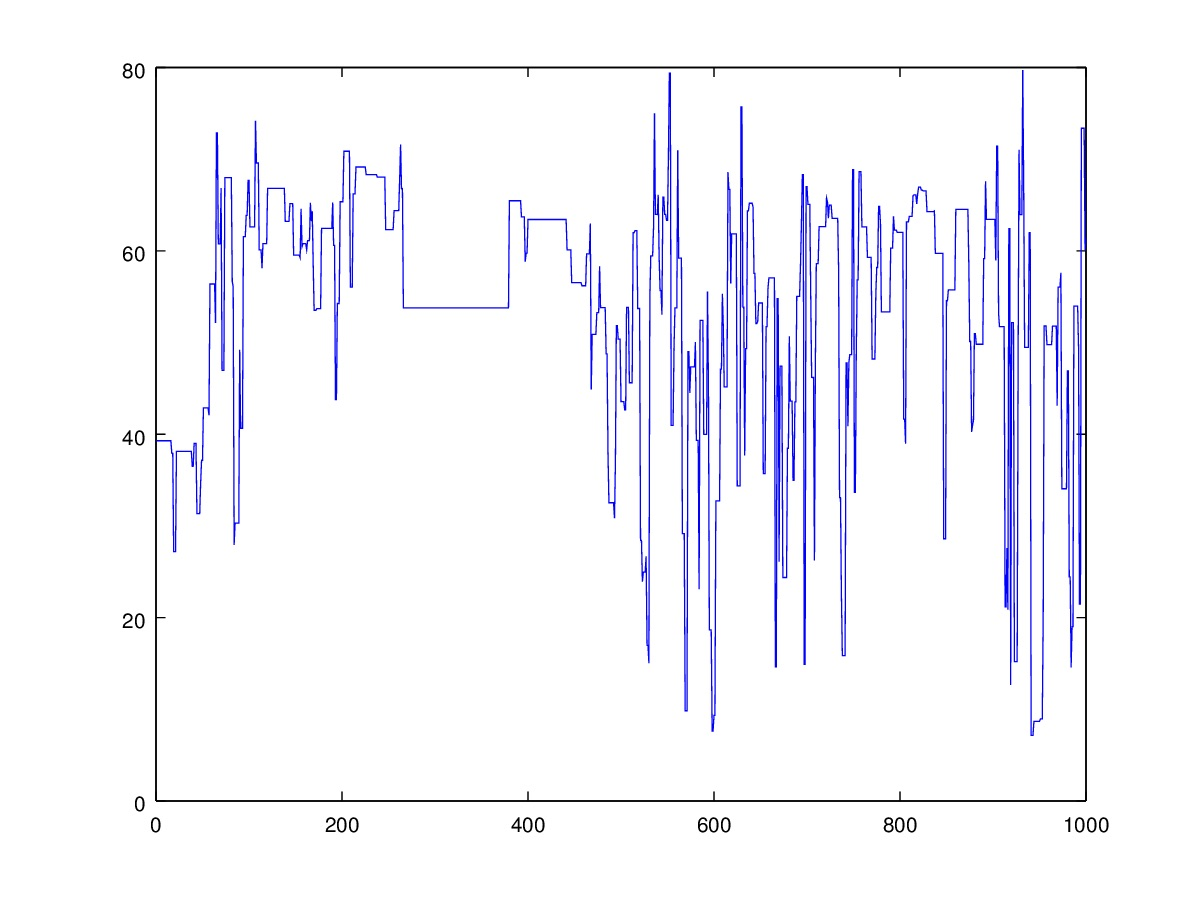
\includegraphics[keepaspectratio,width=0.9\textwidth]{method4.jpg}

\caption{Model 4: Angle between $\bm{g}$ and $\bm{p}$ between successive iterations}

\label{fig:method4}

\end{figure}

After $K$ tournaments, the modelling is same as in the previous subsection:

\begin{equation}
\begin{aligned}
p(\bm{\alpha},\bm{\beta}|\mathbf{g}) &\propto \int p(k|\bm{\alpha},\bm{\beta},\mathbf{g},\mathbf{p},q) p(\mathbf{p}|\bm{\alpha},\bm{\beta}) p(\bm{\alpha},\bm{\beta})p(q) \, \mathrm{d}\mathbf{p} \,  \mathrm{d}q \\
p(\bm{\alpha},\bm{\beta}|\mathbf{g}) &\propto \int Binomial(k|\bm{\alpha},\bm{\beta},\mathbf{g},\mathbf{p},q) Beta(\mathbf{p}|\bm{\alpha},\bm{\beta}) p(\bm{\alpha},\bm{\beta})p(q) \, \mathrm{d}\mathbf{p} \,  \mathrm{d}q
\end{aligned}
\end{equation}


\section{Results (work in progress)}
\label{results}

Metropolis-Hastings Monte Carlo sampling was used as a basis of our work to sample from the proposed distributions with 1000 and 10000 steps forward. Integrals were approximated using N=100 samples from distributions without estimating confidence bounds for mean values. The number of genes (dimensions) was kept low at 3 in order to make computations tractable using laptop computers.

Initial analysis of the results showed, despite theoretical calculations, that discretization of age to different variables was not a successful strategy for learning correct parameters in the simulations.



\section{Conclusions} \label{conclusions}

The keypoint is that in order to get good results and avoid getting stuck into local minimas, one needs to support individuals sampling low probability regions/tails of the distribution. If the individuals in low probability regions die, then the search and transfer of information doesn't happen as fast as possible and the group is likely to lose against other groups which are able to collect and process information faster. This means weaker individuals (risk takers) should be supported somehow in order to maintain the whole distribution and the inference/optimization rule. For example, stronger individuals (having enough intelligence) may gain extra information by observing and learning from mistakes of others. 

However, this theoretical framework partially ignores generation of descendants through sex and is best suited for species which reproduces through mutation. Mutations  happen in a distributed fashion without central control and the process is similar to MCMC sampling. Further work could involve improved modelling, computer simulations and documenting how adaptation speed and quality varies as a function of death probability for low fitness individuals, and how the use of only life expectancy as the fitness function, and not the competition, changes information transfer rates from environment.

\begin{thebibliography}{9}

\bibitem{infobook03}
  MacKay D.,
  \emph{Information Theory, Inference and Learning Algorithms},
  Cambridge University Press,
  2003.

\bibitem{bdanalysis03}
  Gelman A., Carlin J., Stern H. and Rubin D.,
  \emph{Bayesian Data Analysis. 2nd edition.},
  CRC Press, 
  2003.

\bibitem{strens03}
  Strens M.,
  \emph{Evolutionary MCMC Sampling and Optimization in Discrete Spaces},
  Proceedings of The Twentieth International Conference of Machine Learning,
  2003.

\bibitem{entropy01}
  Beirlant J., Dudewicz E., Györfi L., van der Meulen E.,
  \emph{Nonparametric entropy estimation: an overview},
  2001.

\end{thebibliography}

\appendix
\section{Information Theory}

It is almost trivial to prove equation \ref{entropyupdate} is correct from bayesian update equation \ref{bayesupdate}.

\begin{equation*}
\begin{aligned}
p(\bm{x}|\bm{f})p(\bm{f}) &= p(\bm{f}|\bm{x})p(\bm{x})\\
H(\bm{X}|\bm{F})+H(\bm{F}) &= H(\bm{X},\bm{F}) \\
H(\bm{X}|\bm{F}) &= H(\bm{X},\bm{F}) - H(\bm{F}) \\
H(\bm{X}|\bm{F}) &= H(\bm{X}) - I(\bm{X};\bm{F})
\end{aligned}
\end{equation*}

It is important to remember that while entropy measures average  information coding length, it not always the best way to compare, for example, distributions as direct  Kullback-Leibler divergence is not very good at comparing similarity of two distributions. In case of KL divergence, this can be partly remedied by taking absolute value of logarithms meaning that maximum of distribution ratios are used and a coding length of value cannot make up differences in coding lengths of another values etc.

\end{document}

